
\documentclass[11pt,a4paper]{article}
\usepackage[margin=1in]{geometry}
\usepackage{graphicx}
\usepackage{booktabs}
\usepackage{tabularx}
\usepackage{longtable}
\usepackage{array}
\usepackage{hyperref}
\usepackage{float}
\usepackage{caption}
\usepackage{xcolor}
\usepackage{enumitem}
\usepackage{microtype}
\usepackage{url}
\setlist{nosep}
\hypersetup{colorlinks=true,linkcolor=black,urlcolor=blue,citecolor=black}
\newcolumntype{Y}{>{\raggedright\arraybackslash}X}
\title{From Current BOAMP Notices to Procurement-Recurrence Risk:\\A Current Enriched Proxy-Event and Survival-Analysis Framework for Gigalis}
\author{Gigalis internship project}
\date{Generated from current executed outputs on 2026-07-09T14:50:19+00:00}

\begin{document}
\maketitle

\begin{abstract}
This report replaces the earlier 2015--2024 synthesis with a current enriched BOAMP study. It keeps the rich methodological structure of the previous draft, but every headline number is rebuilt from the current files under \protect\path{data/processed/boamp_current/} and current report tables. The event is a proxy recurrence, meaning an identifiable reappearance of a similar procurement need in BOAMP; it is not a legally verified renewal.
\end{abstract}

\tableofcontents
\clearpage

\section{Executive Summary}
Gigalis needs a practical way to monitor public digital procurement needs before they reappear in BOAMP. The current enriched dataset covers 2015-03-02 to 2026-07-09 and contains 3,656 retained BOAMP notices. Within that source, 2,216 are APPEL\_OFFRE notices. After start-date and duration eligibility rules, 1,661 contracts are eligible for recurrence linkage.

The current selected event definition is \textbf{M0 balanced}. It produces 183 proxy recurrence events and 1,478 censored contracts, an event rate of 11.0\%. M2 balanced has the strongest current synthetic/silver F1 (0.928) and very high precision, but it keeps only 68 events. The current selection therefore keeps M0 balanced as the main operational survival definition because it has enough events for survival modeling, transparent thresholds, zero current negative-control acceptance, and stable interpretation.

Under the selected definition, Kaplan--Meier survival is 95.5\% at 12 months, 94.4\% at 24 months, 90.2\% at 48 months, and 87.7\% at 60 months. The current Cox model has C-index 0.720; the selected AFT model is LogLogisticAFT with AIC 2676.5. The live scoring table covers 1,661 contracts and gives mean p12/p24 of 0.029/0.051, corresponding to 48.4 expected proxy recurrences within 12 months and 84.6 within 24 months.

\section{Business Context and Interpretation}
The study supports account monitoring and segment planning. It does not try to prove a legal renewal chain. BOAMP does not contain a complete contract-history identifier linking each call for tender to later renewals. The output is therefore a prioritization layer: it identifies plausible, observable reappearances of similar digital procurement needs.

The distinction matters operationally. A high p12 or p24 score means that under the selected proxy-event definition and fitted survival model, a similar BOAMP notice is relatively likely to be observed soon. It does not mean that the buyer has a legal obligation to renew, that an incumbent contract will be extended, or that a future notice is guaranteed.

\section{Current Data Source and Study Period}
The downloader used the BOAMP Opendatasoft API, Pays de la Loire departments, and digital CPV divisions. It requested 2015-01-01 to 2026-07-09 and retained a verified actual date range of 2015-03-02 to 2026-07-09. Raw JSON pages and metadata are cached under \protect\path{data/raw/boamp_current/} and the flattened current source is \protect\path{data/processed/boamp_current/boamp_full_flat.csv}.

\begin{table}[H]
\centering
\caption{Current analytical population funnel. Source: \protect\path{reports/tables/data/analytical_population_summary.csv}.}
\begin{tabular}{lrl}
\toprule
Stage & Rows & Interpretation \\
\midrule
All current notices & 3,656 & downloaded and deduplicated BOAMP notices \\
APPEL\_OFFRE notices & 2,216 & survival source unit \\
APPEL\_OFFRE with valid source date & 2,215 & usable start date before censoring \\
Eligible for linkage & 1,661 & expected end date plus search buffer before censoring \\
\bottomrule
\end{tabular}
\end{table}

\begin{figure}[H]
\centering
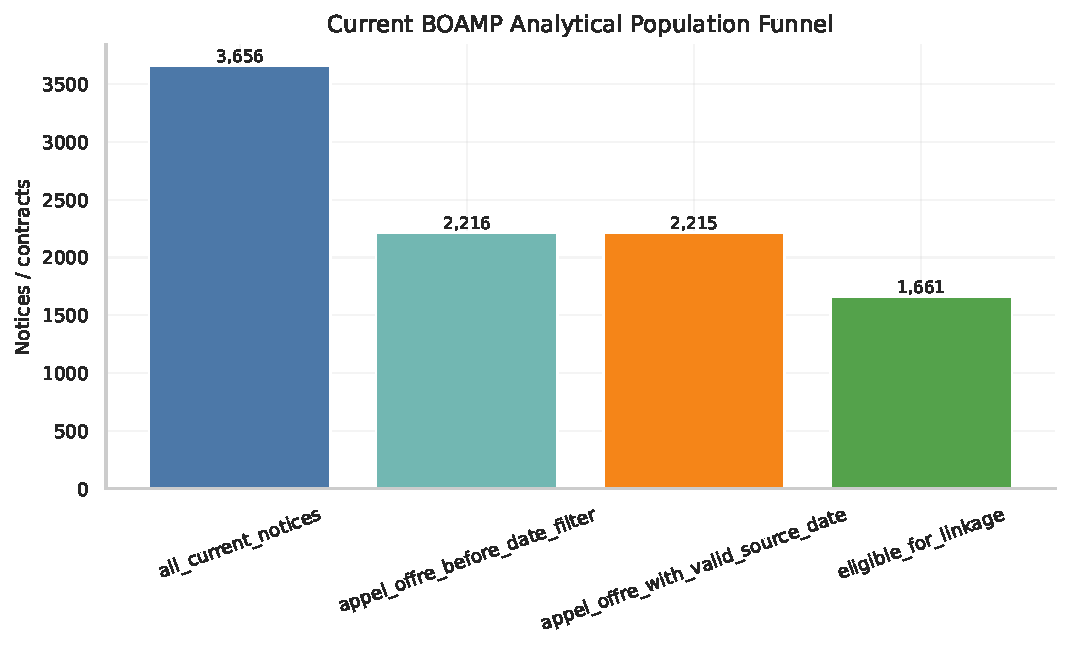
\includegraphics[width=.82\linewidth]{figures/data/analytical_population_funnel.pdf}
\caption{Current analytical population funnel generated from the refreshed pipeline.}
\end{figure}

\section{SIREN/SIRET Enrichment and Buyer-Key Construction}
The current cleaning pipeline preserves raw buyer names and raw identifiers, then builds cleaned SIRET, cleaned SIREN, SIREN extracted from SIRET, and high-confidence enriched SIREN when possible. The buyer key is assigned in this order: valid SIRET, valid SIREN, SIREN extracted from SIRET, enriched SIREN, and finally normalized-name fallback.

The refreshed dataset has 480 rows with valid SIRET and 2,535 rows with enriched SIREN. Buyer-key quality is central because it controls the blocking step: better buyer grouping increases the chance of finding plausible later notices without opening the candidate pool to unrelated buyers.

\begin{table}[H]
\centering
\caption{Buyer-key distribution in the current enriched dataset. Source: \protect\path{reports/tables/data/buyer_key_quality_summary.csv}.}
\begin{tabular}{lrr}
\toprule
Buyer key type & Rows & Distinct buyer keys \\
\midrule
NAME & 930 & 202 \\
SIREN\_ENRICHED & 2,246 & 216 \\
SIRET & 480 & 132 \\
\bottomrule
\end{tabular}
\end{table}

\section{Cleaning, Duration, CPV, and Traceability}
The current dataset normalizes notice identifiers, publication dates, nature, buyer names, SIRET/SIREN, CPV, procurement-object text, duration, and source-date fields. CPV is converted into a cleaned code, hierarchy fields, and generic-CPV flags. Generic codes are treated cautiously because a broad code can make two notices look more similar than they really are. Duration is preserved when plausible and imputed when missing or suspect; the imputation flag remains available downstream so survival models can account for this uncertainty.

Traceability is kept at every stage: raw notice IDs and raw-record fields are preserved in the enriched table, candidate-pair files keep both source and candidate identifiers, selected event datasets keep the method definition, and report values are traced in \protect\path{reports/current_source_values_used.csv} and \protect\path{reports/final_draft/source_values_used.csv}.

\section{Candidate-Pair Generation}
Candidate pairs are generated within the enriched buyer key. A source APPEL\_OFFRE can link only to a later notice from the same buyer key, and the search window is centered around the expected end date. The candidate table includes text similarity, CPV compatibility, temporal proximity, buyer-key quality, generic-CPV flags, duration features, candidate rank, score margin, and the text backend. The refreshed run used sentence\_transformers:paraphrase-multilingual-MiniLM-L12-v2.

\begin{table}[H]
\centering
\caption{Current candidate generation summary. Source: \protect\path{reports/tables/linkage/candidate_generation_summary.csv}.}
\begin{tabular}{lr}
\toprule
Metric & Value \\
\midrule
Eligible source contracts & 1,661 \\
Candidate pairs & 7,699 \\
Sources with at least one candidate & 945 \\
Text similarity backend & sentence\_transformers:paraphrase-multilingual-MiniLM-L12-v2 \\
\bottomrule
\end{tabular}
\end{table}

\begin{figure}[H]
\centering
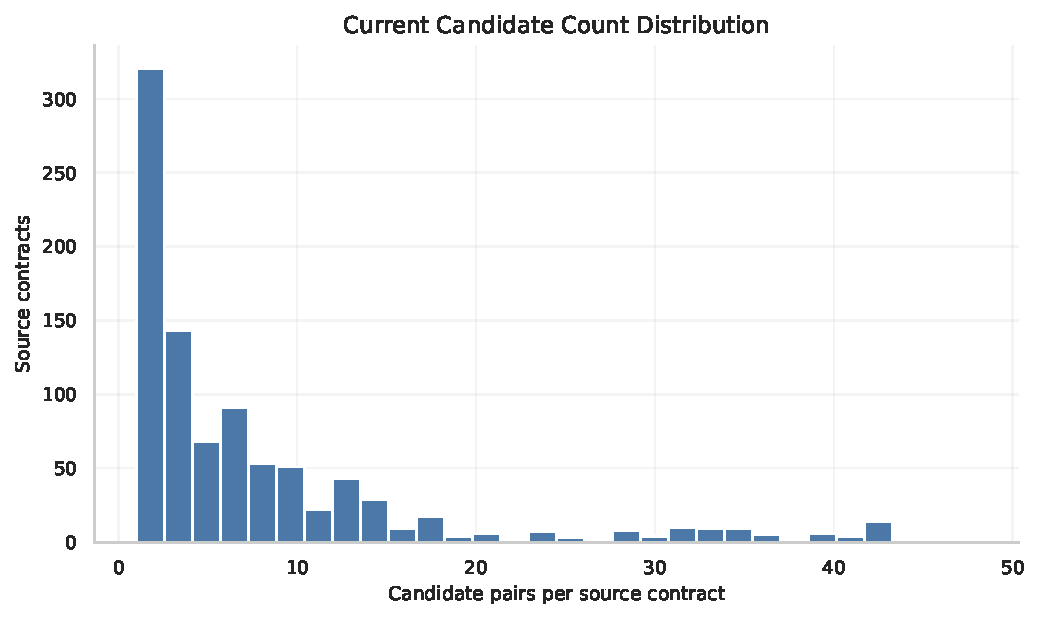
\includegraphics[width=.78\linewidth]{figures/linkage/candidate_count_distribution.pdf}
\caption{Distribution of candidate counts per eligible source contract.}
\end{figure}

\section{No-Ground-Truth Validation Framework}
Real BOAMP does not provide true recurrence-chain labels. This study therefore uses several imperfect but complementary diagnostics:
\begin{enumerate}
\item synthetic/silver labels to estimate precision, recall, and F1 under controlled conditions;
\item negative-control acceptance to detect implausible false-positive behavior;
\item external-reference diagnostics such as ATTRIBUTION \protect\path{annonce_lie} only as weak signals;
\item subgroup audits for generic CPV, name-fallback buyers, imputed durations, near-threshold links, and low-margin links;
\item unique-link diagnostics to identify candidate notices reused too often.
\end{enumerate}

\begin{figure}[H]
\centering
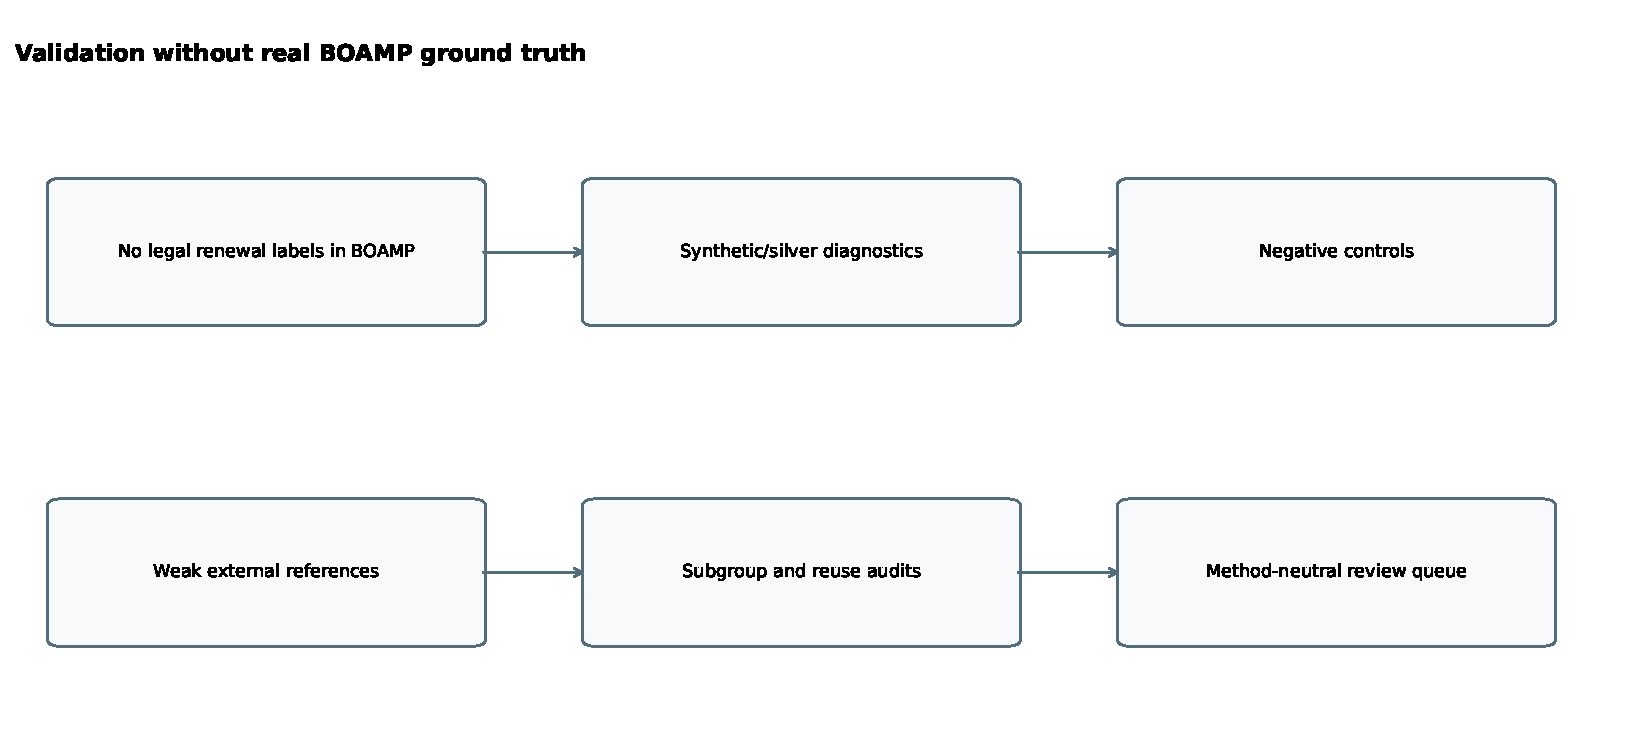
\includegraphics[width=.92\linewidth]{final_draft/figures/fig_no_ground_truth_validation_framework.pdf}
\caption{Validation logic for BOAMP recurrence when real legal renewal ground truth is unavailable.}
\end{figure}

\section{M0, M1, and M2 Linkage Methods}
M0 is the deterministic composite-rule family. It is transparent and easy to audit: the selected balanced variant applies text, composite score, margin, and generic-CPV logic directly. M1 is a probabilistic classifier over the current pair features. M2 is the probability/review-zone variant: it performs very well on synthetic/silver labels but is intentionally stricter in the current data.

\begin{table}[H]
\centering
\caption{Current M0/M1/M2 method comparison. Synthetic/silver metrics are diagnostics, not real BOAMP truth.}
\small
\resizebox{\linewidth}{!}{%
\begin{tabular}{lrrrrrrr}
\toprule
Method & Events & Event rate & Precision & Recall & F1 & Neg. control & Generic CPV \\
\midrule
M0 balanced & 183 & 11.0\% & 0.377 & 0.986 & 0.545 & 0.0\% & 7.7\% \\
M0 broad & 447 & 26.9\% & 0.157 & 1.000 & 0.271 & 0.0\% & 13.6\% \\
M0 strict & 87 & 5.2\% & 0.529 & 0.657 & 0.586 & 0.0\% & 0.0\% \\
M1 balanced & 173 & 10.4\% & 0.393 & 0.971 & 0.560 & 1.2\% & 2.3\% \\
M2 balanced & 68 & 4.1\% & 0.941 & 0.914 & 0.928 & 0.0\% & 0.0\% \\
\bottomrule
\end{tabular}
}
\end{table}

\begin{figure}[H]
\centering
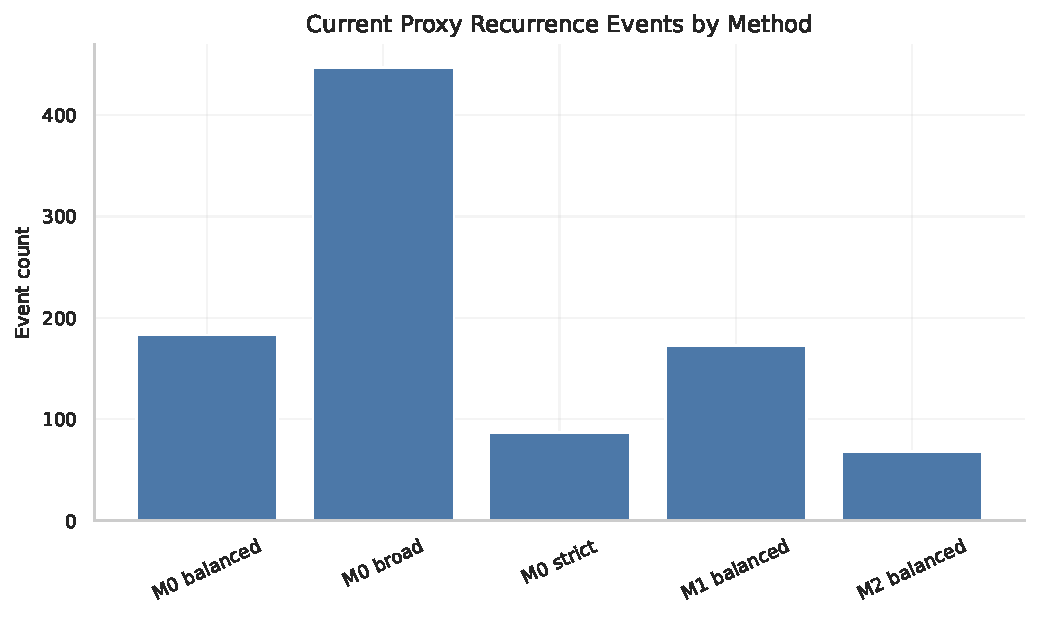
\includegraphics[width=.78\linewidth]{figures/linkage/method_event_counts.pdf}
\caption{Current proxy recurrence event counts by method.}
\end{figure}

\begin{figure}[H]
\centering
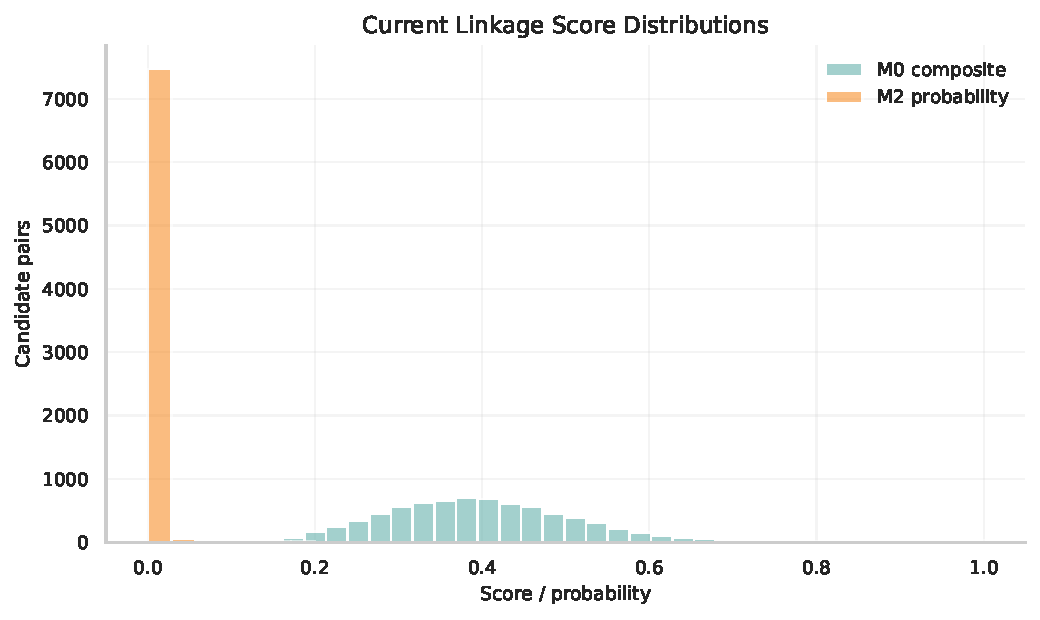
\includegraphics[width=.78\linewidth]{figures/linkage/method_score_distributions.pdf}
\caption{Current score/probability distributions by method.}
\end{figure}

\section{Methodology Tests Inspired by Record Linkage Literature}
The refreshed methodology tables test classifier alternatives, blocking alternatives, text-similarity alternatives, threshold zones, active-learning label budgets, subgroup quality, unique-link reuse, and weak external references. The classifier benchmark does not treat BOAMP as ground truth; it uses current synthetic/silver labels and real-data diagnostics.

\begin{table}[H]
\centering
\caption{Current classifier benchmark. LightGBM is blocked by a missing system OpenMP library and is not used as selection evidence.}
\small
\begin{tabular}{llrrr}
\toprule
Model & Status & Precision & Recall & F1 \\
\midrule
lightgbm & blocked & -- & -- & -- \\
M0 balanced & run & 0.189 & 1.000 & 0.317 \\
logistic\_regression & run & 0.322 & 0.971 & 0.484 \\
random\_forest & run & 0.904 & 0.943 & 0.923 \\
gradient\_boosting & run & 0.952 & 0.857 & 0.902 \\
svm\_rbf & run & 0.828 & 0.757 & 0.791 \\
xgboost & run & 0.957 & 0.943 & 0.950 \\
Fellegi-Sunter/recordlinkage & available\_diagnostic & 0.189 & 1.000 & 0.317 \\
Splink & available\_diagnostic & 0.941 & 0.914 & 0.928 \\
\bottomrule
\end{tabular}
\end{table}

Threshold-zone diagnostics are retained for review prioritization rather than replacing the final event definition. The current possible-match zone contains 14 candidate pairs and the strong-match zone contains 68; this distinction is useful for future manual review queues.

\section{Final Selected Proxy-Event Definition}
The selected current event definition is \textbf{M0 balanced}. It is not selected because it maximizes benchmark F1. It is selected because the current study needs a survival-ready event definition that balances event sufficiency, interpretability, negative-control behavior, generic-CPV risk, and operational stability.

M2 balanced is important evidence, not the selected survival input. It has F1 0.928, precision 0.941, recall 0.914, zero generic-CPV share, and 68 events. That is excellent as a strong-match / review-priority layer, but too sparse to replace the selected event definition in the current survival study without making the event count fragile. The selected M0 balanced definition keeps 183 events, zero current negative-control acceptance, and readable rule logic.

\section{Survival-Analysis Methodology}
The survival unit remains APPEL\_OFFRE. Each eligible source contract receives an observed duration: either time to selected proxy recurrence, or time to censoring if no selected proxy recurrence is observed. Kaplan--Meier estimates the nonparametric survival curve. Cox PH is used as a ranking and covariate diagnostic. AFT models compare parametric time-to-event shapes and provide the operational p12/p24 scoring layer.

\begin{figure}[H]
\centering
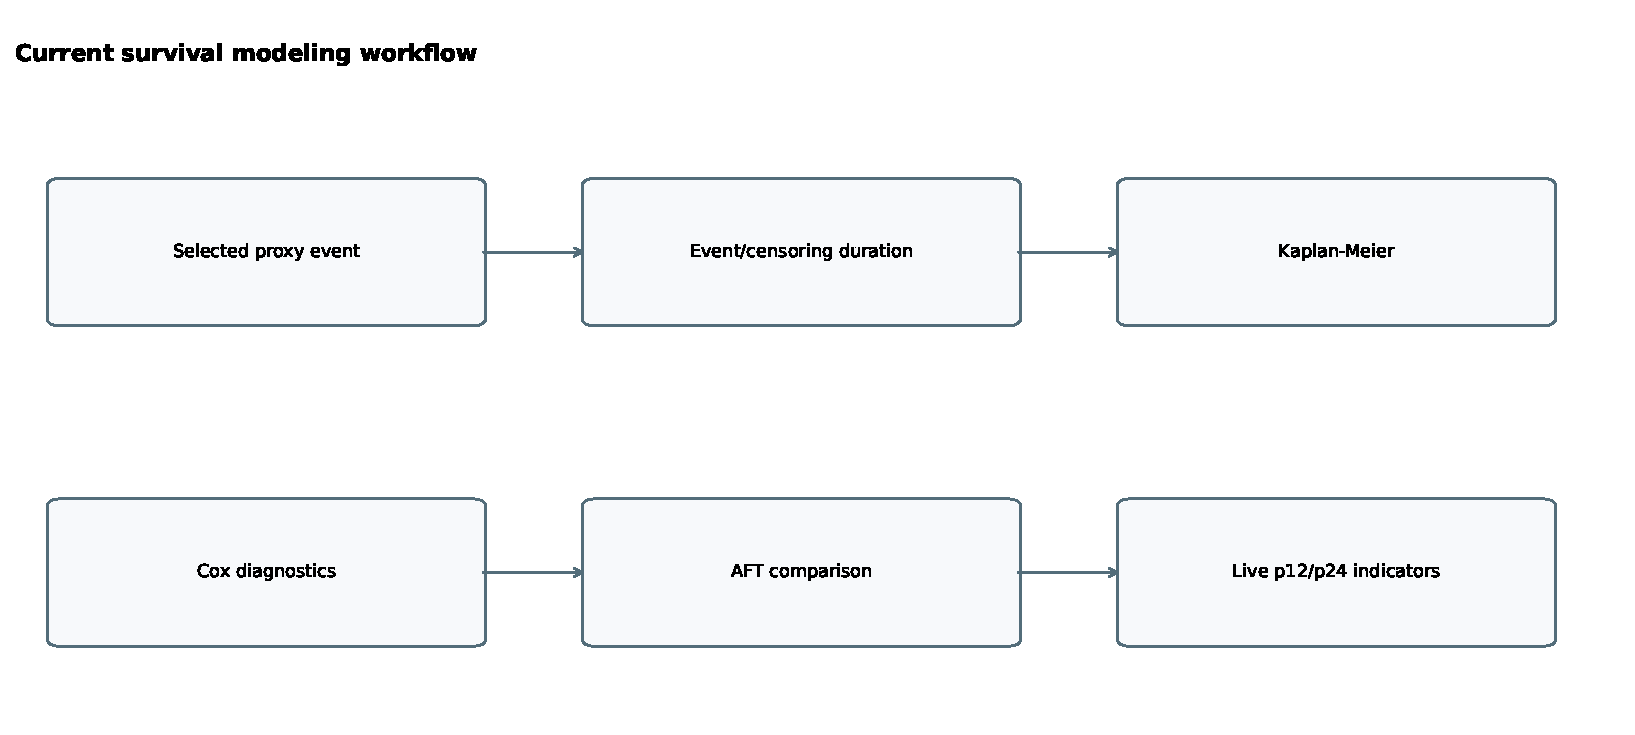
\includegraphics[width=.9\linewidth]{final_draft/figures/fig_survival_modeling_workflow.pdf}
\caption{Current survival modeling workflow from selected proxy-event definition to operational p12/p24 indicators.}
\end{figure}

\section{Current Survival Results}
Under M0 balanced, there are 183 proxy recurrence events among 1,661 eligible contracts. The Kaplan--Meier median is not reached, because fewer than half of contracts experience the selected proxy recurrence before censoring. Survival remains high at the first operational horizons: 95.5\% at 12 months and 94.4\% at 24 months.

\begin{table}[H]
\centering
\caption{Current survival headline results. Source: \protect\path{reports/tables/survival/survival_summary_current.csv}.}
\begin{tabular}{lrrrrr}
\toprule
Method & Events & Event rate & S12 & S24 & S60 \\
\midrule
M0 balanced & 183 & 11.0\% & 95.5\% & 94.4\% & 87.7\% \\
\bottomrule
\end{tabular}
\end{table}

\begin{figure}[H]
\centering
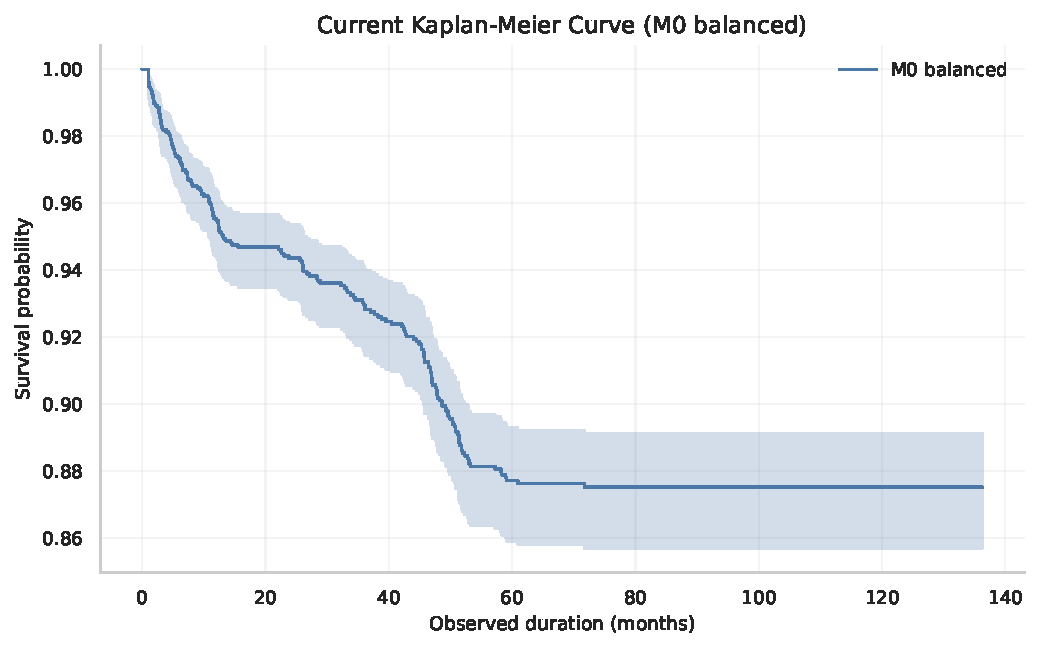
\includegraphics[width=.78\linewidth]{figures/survival/km_curve_current.pdf}
\caption{Kaplan--Meier curve under the selected current proxy-event definition.}
\end{figure}

\section{Cox and AFT Model Diagnostics}
The current Cox model C-index is 0.720. Duration has a negative coefficient, meaning longer declared duration is associated with lower short-term recurrence hazard in the fitted model. Buyer-key type and segment terms are retained as diagnostics, not causal effects.

\begin{table}[H]
\centering
\caption{Selected Cox coefficients. Source: \protect\path{reports/tables/survival/cox_results_current.csv}.}
\small
\begin{tabular}{lrrr}
\toprule
Variable & Coef. & Hazard ratio & p-value \\
\midrule
declared\_duration\_months & -0.012 & 0.988 & 8.35e-05 \\
duration\_imputed\_flag & 0.019 & 1.019 & 0.892 \\
start\_year & -0.004 & 0.996 & 0.836 \\
segment\_model\_IT Services \& Consulting & 0.232 & 1.261 & 0.0588 \\
segment\_model\_Other & 0.039 & 1.040 & 0.808 \\
segment\_model\_Software \& Applications & -0.264 & 0.768 & 0.0848 \\
segment\_model\_Telecom \& Networks & -0.013 & 0.987 & 0.927 \\
segment\_model\_Unknown & -0.055 & 0.946 & 0.768 \\
\bottomrule
\end{tabular}
\end{table}

The selected AFT model is LogLogisticAFT. The AFT comparison is useful because fixed-horizon operational probabilities require a full predicted survival curve, not only a relative hazard ranking.

\begin{table}[H]
\centering
\caption{Current AFT model comparison. Source: \protect\path{reports/tables/survival/aft_comparison_current.csv}.}
\begin{tabular}{lrr}
\toprule
Model & AIC & Events \\
\midrule
LogLogisticAFT & 2676.5 & 183 \\
WeibullAFT & 2680.8 & 183 \\
LogNormalAFT & 2757.6 & 183 \\
\bottomrule
\end{tabular}
\end{table}

\begin{figure}[H]
\centering
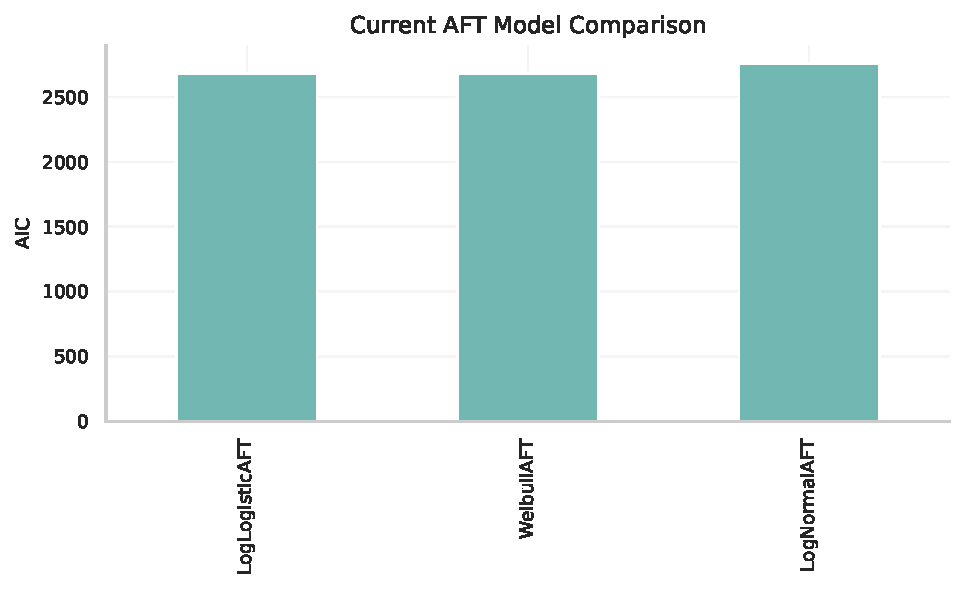
\includegraphics[width=.78\linewidth]{figures/survival/aft_model_comparison_current.pdf}
\caption{AFT comparison under the selected current event definition.}
\end{figure}

\section{Operational 12/24-Month Indicators}
The operational layer scores contracts by conditional p12 and p24 under the selected AFT model. These are prioritization scores for visible BOAMP proxy recurrences. Mean p12 is 0.029, mean p24 is 0.051, and the expected current workload is 48.4 proxy recurrences in 12 months and 84.6 in 24 months.

\begin{figure}[H]
\centering
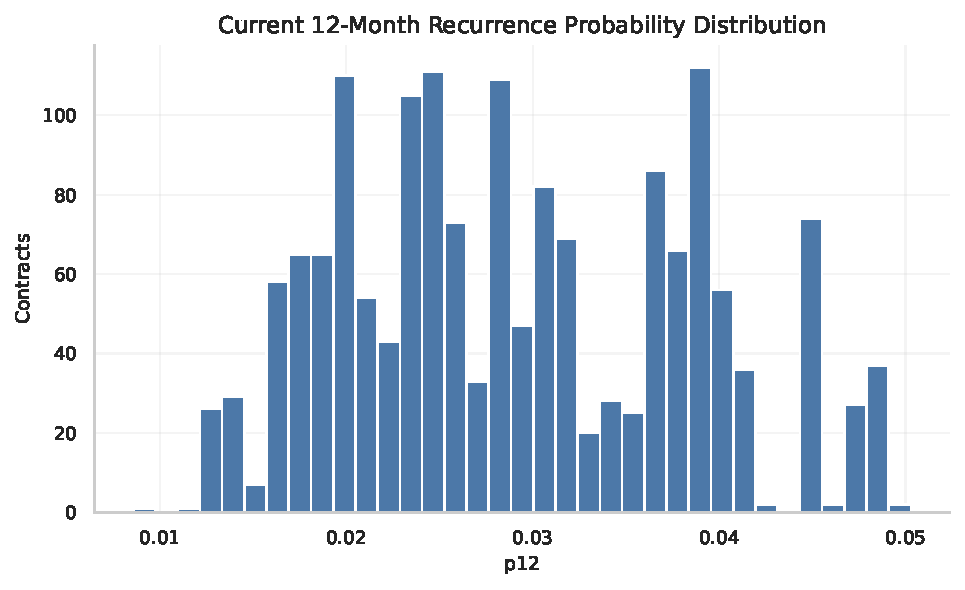
\includegraphics[width=.78\linewidth]{figures/survival/p12_distribution_current.pdf}
\caption{Distribution of current 12-month proxy-recurrence probabilities.}
\end{figure}

\begin{table}[H]
\centering
\caption{Top buyer-level expected proxy recurrences. Source: \protect\path{reports/tables/survival/buyer_risk_ranking_current.csv}.}
\small
\begin{tabular}{llrrr}
\toprule
Buyer key & Buyer name & Contracts & Expected 12m & Expected 24m \\
\midrule
SIREN:234400034 & Conseil régional des Pays de la Loire & 93 & 3.17 & 5.53 \\
SIREN:794304097 & Nantes Métropole & 93 & 2.42 & 4.24 \\
SIREN:264400136 & CHU de Nantes & 51 & 1.47 & 2.56 \\
SIREN:228500013 & Département de la Vendée & 31 & 1.13 & 1.97 \\
SIREN:244900015 & Angers Loire Métropole & 35 & 1.10 & 1.91 \\
SIREN:391722881 & GIE SESAM Vitale & 32 & 1.07 & 1.86 \\
SIREN:935367433 & Conseil départemental Loire-Atlantique & 29 & 1.03 & 1.79 \\
SIREN:194909701 & Université d'Angers & 30 & 0.88 & 1.54 \\
\bottomrule
\end{tabular}
\end{table}

\begin{table}[H]
\centering
\caption{Top segment-level expected proxy recurrences. Source: \protect\path{reports/tables/survival/segment_risk_ranking_current.csv}.}
\small
\begin{tabular}{lrrrr}
\toprule
Segment & Contracts & Expected 12m & Expected 24m & Mean p12 \\
\midrule
IT Services \& Consulting & 478 & 16.29 & 28.35 & 0.034 \\
Telecom \& Networks & 300 & 8.60 & 15.02 & 0.029 \\
Cybersecurity & 199 & 6.03 & 10.54 & 0.030 \\
Software \& Applications & 295 & 6.00 & 10.56 & 0.020 \\
Unknown & 165 & 4.77 & 8.34 & 0.029 \\
Digital Workplace \& Collaboration & 72 & 2.09 & 3.65 & 0.029 \\
Data \& AI & 52 & 1.49 & 2.61 & 0.029 \\
IT Hardware \& Equipment & 38 & 1.22 & 2.13 & 0.032 \\
\bottomrule
\end{tabular}
\end{table}

\begin{table}[H]
\centering
\caption{Top contract-level p12/p24 scores. Source: \protect\path{reports/tables/survival/contract_risk_ranking_current.csv}.}
\small
\begin{tabular}{lllrr}
\toprule
Contract & Buyer & Segment & p12 & p24 \\
\midrule
BOAMP:20-100172 & Communauté urbaine d'Alençon & IT Services \& Consulting & 0.050 & 0.087 \\
BOAMP:25-36671 & Direction Cybersécurité, Cloud et IA & IT Services \& Consulting & 0.050 & 0.086 \\
BOAMP:25-50085 & Conseil départemental Loire Atlantique & IT Services \& Consulting & 0.049 & 0.084 \\
BOAMP:25-3181 & Département de la Vendée & IT Services \& Consulting & 0.049 & 0.084 \\
BOAMP:25-28394 & Conseil départemental Loire Atlantique & IT Services \& Consulting & 0.049 & 0.084 \\
BOAMP:25-54937 & Conseil Départemental de la Mayenne & IT Services \& Consulting & 0.049 & 0.084 \\
BOAMP:25-2262 & VILLE DE SAINT NAZAIRE & IT Services \& Consulting & 0.049 & 0.084 \\
BOAMP:25-13579 & Conseil Départemental de la Mayenne & IT Services \& Consulting & 0.049 & 0.084 \\
BOAMP:25-41441 & VILLE DE SAINT NAZAIRE & IT Services \& Consulting & 0.049 & 0.084 \\
BOAMP:24-132180 & Conseil Départemental de la Mayenne & IT Services \& Consulting & 0.049 & 0.084 \\
\bottomrule
\end{tabular}
\end{table}

\begin{figure}[H]
\centering
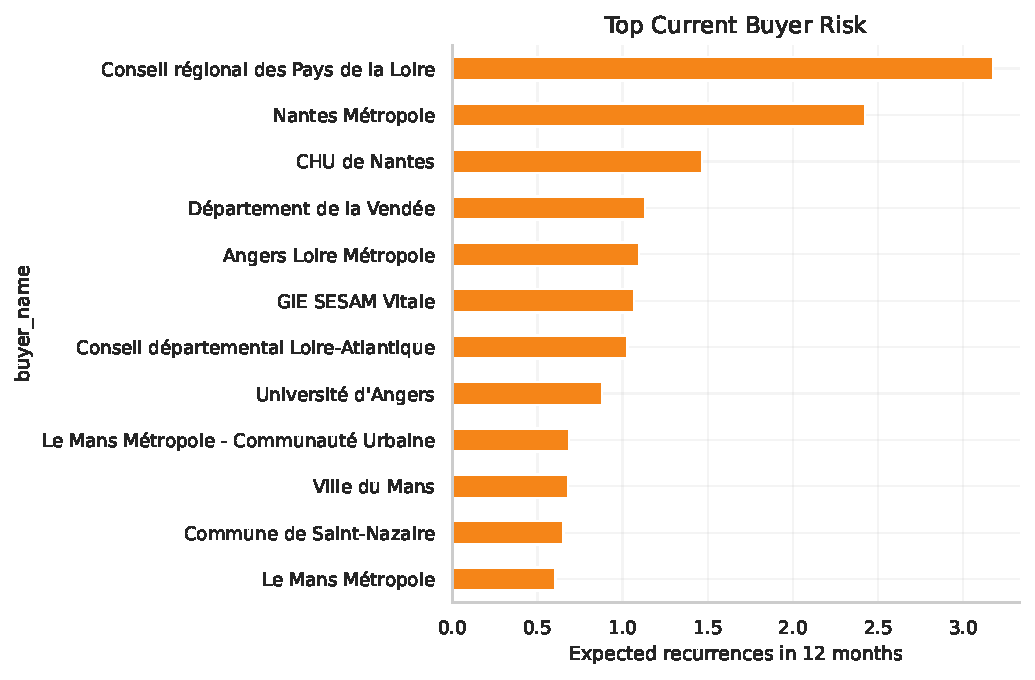
\includegraphics[width=.76\linewidth]{figures/survival/top_buyer_risk_current.pdf}
\caption{Top buyer-level expected 12-month proxy recurrence workload.}
\end{figure}

\begin{figure}[H]
\centering
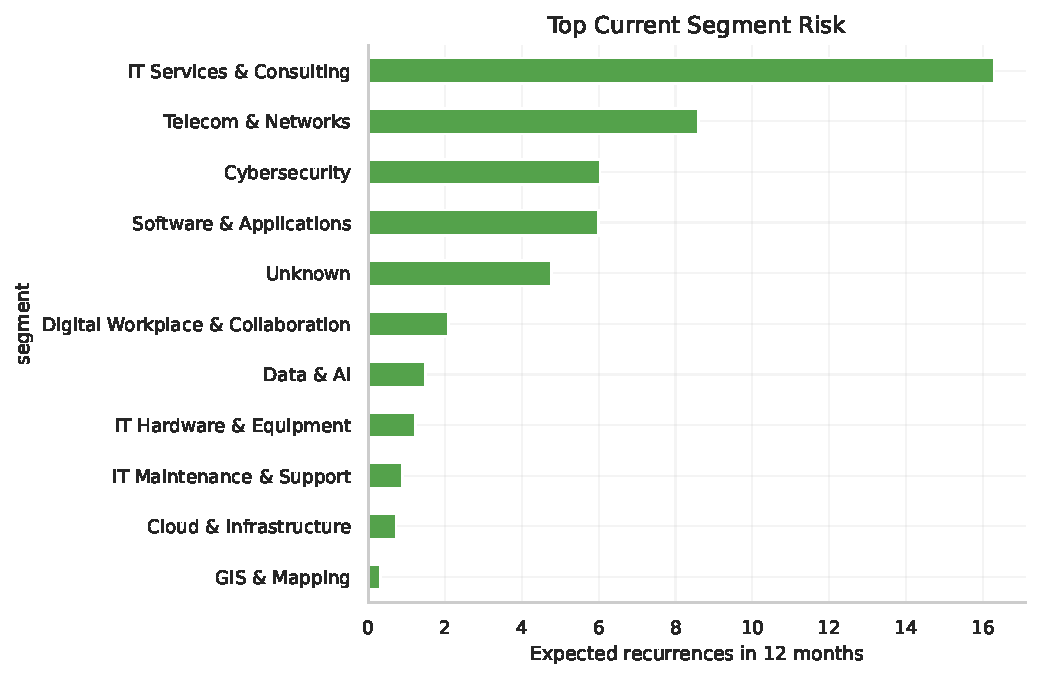
\includegraphics[width=.76\linewidth]{figures/survival/top_segment_risk_current.pdf}
\caption{Top segment-level expected 12-month proxy recurrence workload.}
\end{figure}

\section{Robustness, Review Priorities, and Remaining Risks}
The main review priorities are generic CPV links, name-fallback buyer keys, imputed durations, near-threshold links, low-margin links, and large buyers. Unique-link diagnostics show that some candidate notices are reused many times, with the top reused candidate appearing 13 times. This does not invalidate the method, but it marks those cases for manual review because one later framework-style notice can plausibly be similar to several earlier needs.

\begin{longtable}{p{.28\linewidth}p{.31\linewidth}p{.31\linewidth}}
\caption{Current limitations and mitigations.}\\
\toprule
Limitation & Consequence & Mitigation / current status \\
\midrule
\endfirsthead
\toprule
Limitation & Consequence & Mitigation / current status \\
\midrule
\endhead
No BOAMP legal renewal labels & Real precision and recall are not directly observable & Use proxy wording, synthetic/silver benchmark, negative controls, and review queues \\
M2 is sparse & Strong-match F1 is high but event count is only 68 & Keep M2 as review/strong-match evidence; select M0 balanced for current survival \\
Generic CPV ambiguity & Broad CPV codes can create weak semantic evidence & Flag generic CPV and audit those links first \\
Name-fallback buyers & Residual buyer fragmentation and false grouping risk remain & Continue SIREN/SIRET enrichment and manual buyer checks \\
Duration imputation & Timing uncertainty can affect expected end dates & Preserve duration-imputation flags in linkage and survival outputs \\
LightGBM blocked & One optional classifier benchmark cannot run & Record missing \protect\path{libgomp.so.1} and exclude LightGBM from selection evidence \\
External references are weak & ATTRIBUTION \protect\path{annonce_lie} is not complete ground truth & Use only as diagnostic support, not a label source \\
\bottomrule
\end{longtable}

\section{Conclusion and Next Steps}
The current enriched BOAMP dataset is now the source of truth for this study. The rich report no longer compares old and new results as a main objective. It documents the current data, current enrichment, current linkage, current selected proxy-event definition, current survival outputs, and current operational prioritization layer.

The next substantive work should be method-neutral manual review of possible-match and strong-match zones, targeted review of name-fallback and generic-CPV links, installation or environment support for LightGBM if that benchmark remains desired, and incorporation of reviewed labels into an active-learning loop. The central interpretation should stay conservative: this is a proxy recurrence framework for public BOAMP observability, not a legal renewal detector.

\appendix
\clearpage
\section{Pipeline and Source Trace}
\begin{figure}[H]
\centering
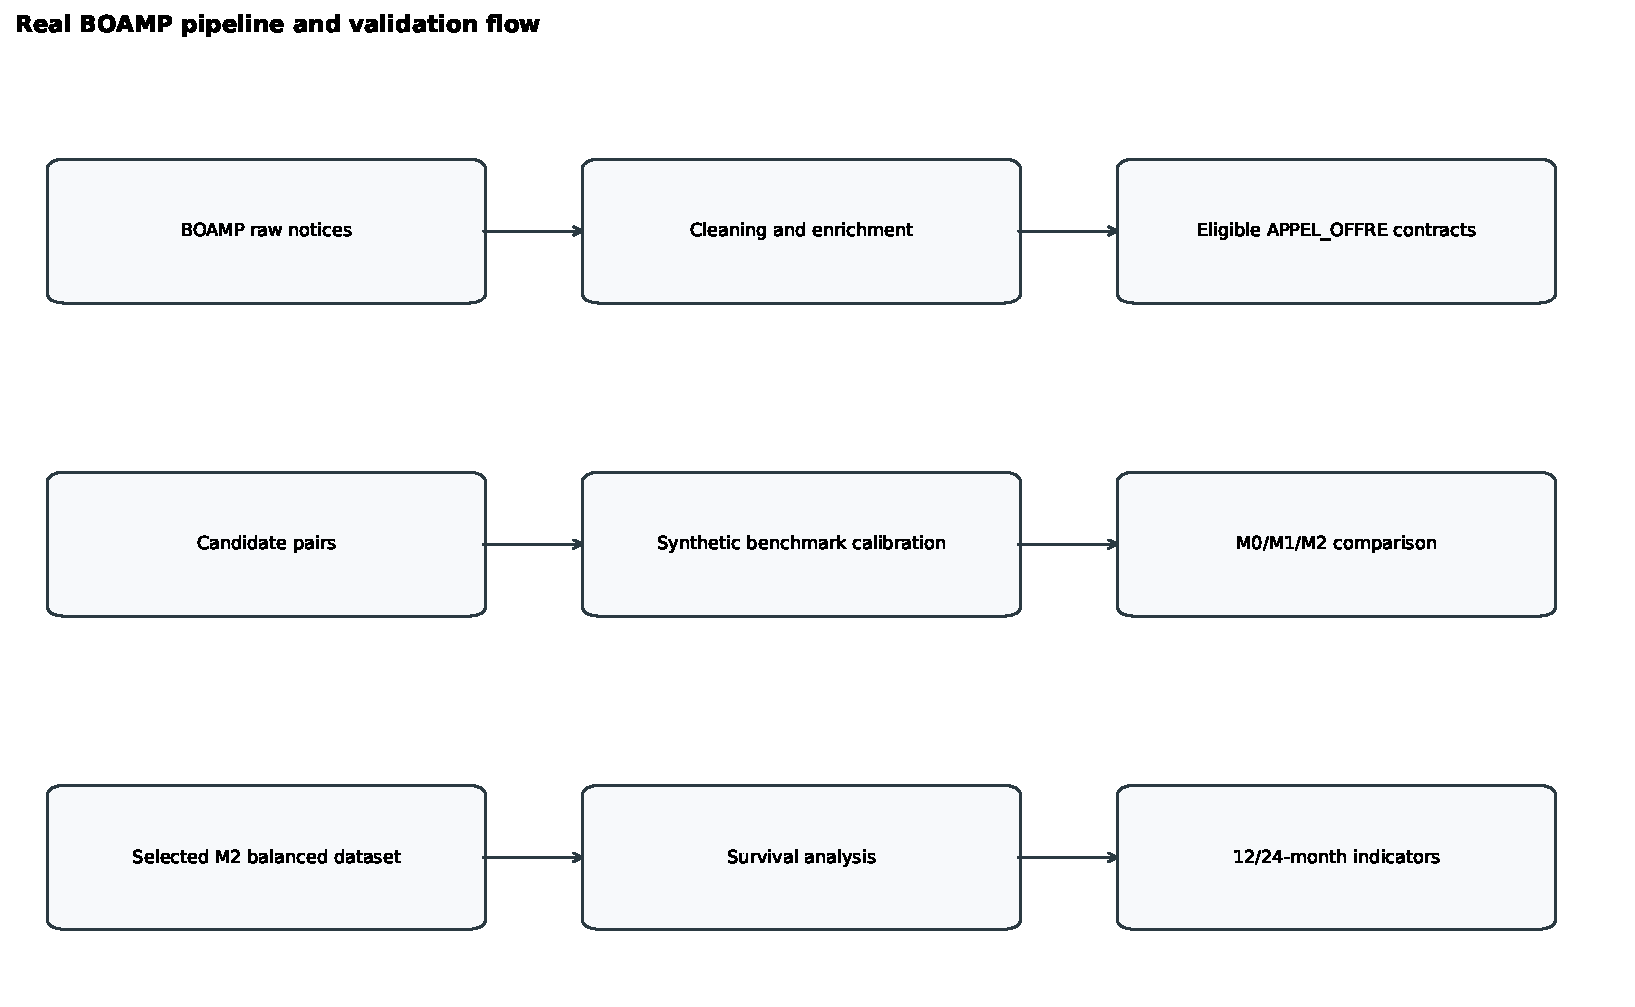
\includegraphics[width=.95\linewidth]{final_draft/figures/fig_pipeline_overview.pdf}
\caption{Current rich-study pipeline from BOAMP download to operational scoring.}
\end{figure}

\begin{figure}[H]
\centering
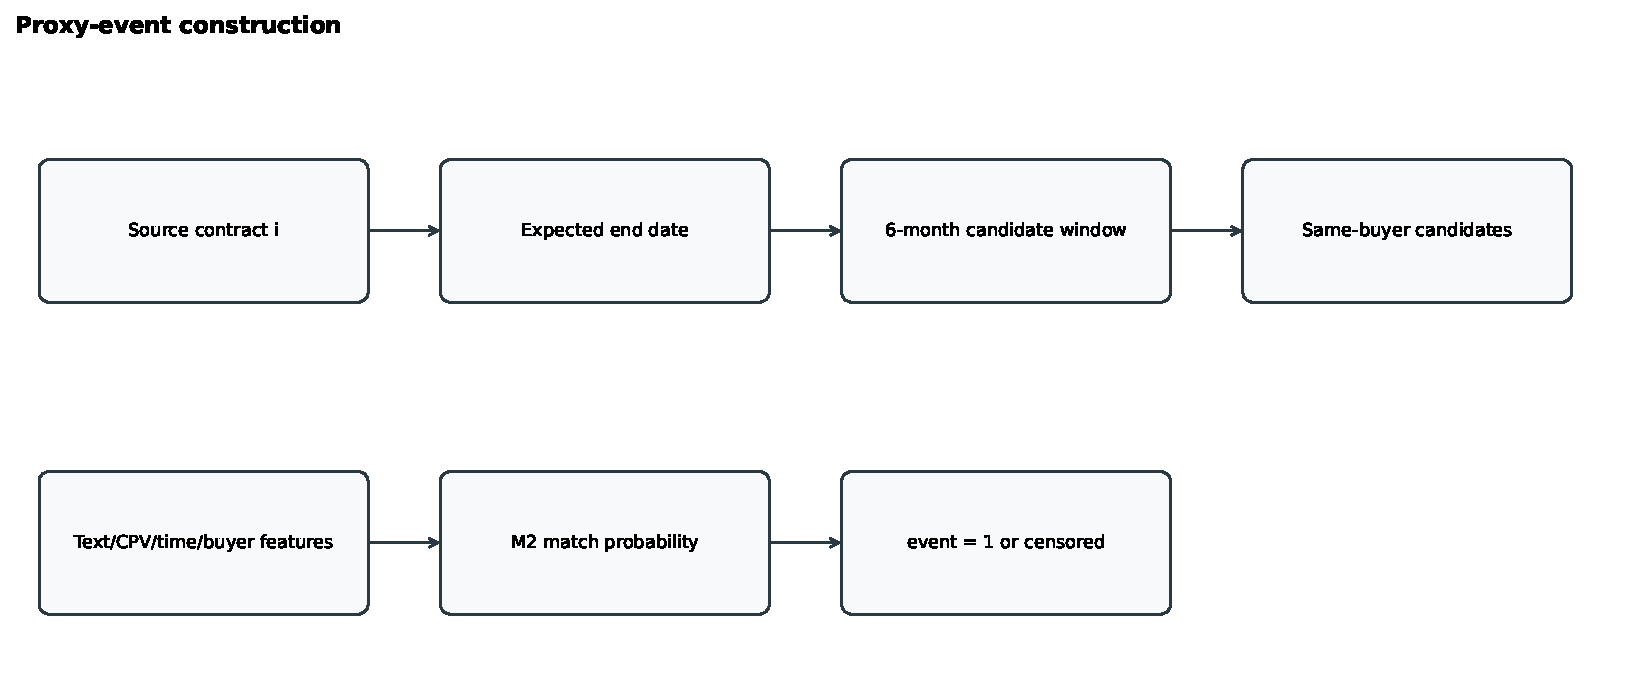
\includegraphics[width=.9\linewidth]{final_draft/figures/fig_proxy_event_construction.pdf}
\caption{Current proxy-event construction logic.}
\end{figure}

\begin{figure}[H]
\centering
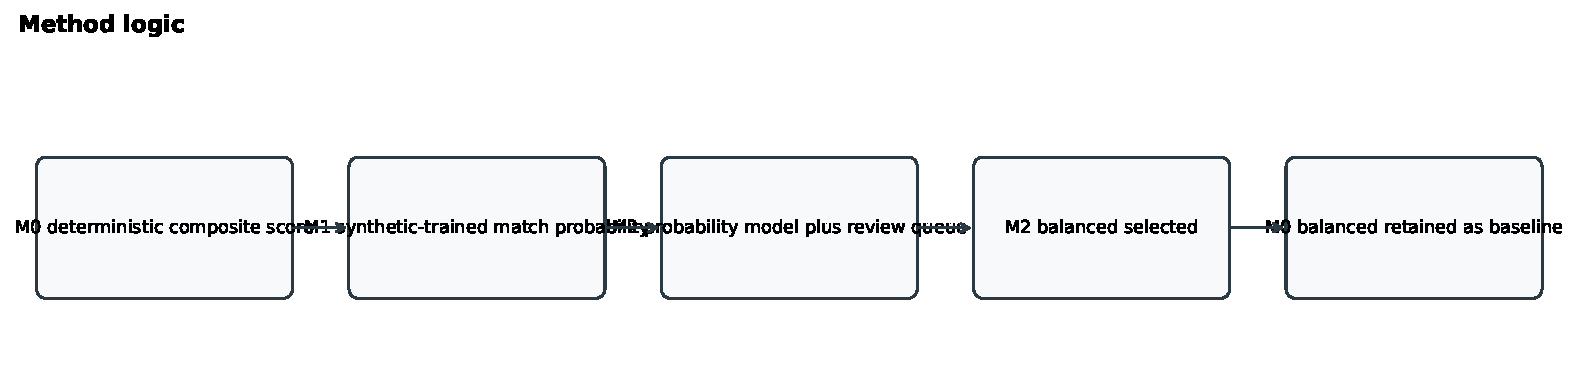
\includegraphics[width=.9\linewidth]{final_draft/figures/fig_m0_m1_m2_method_logic.pdf}
\caption{Current M0/M1/M2 method roles.}
\end{figure}

The complete source trace is stored in \protect\path{reports/current_source_values_used.csv} and \protect\path{reports/final_draft/source_values_used.csv}. The active current report table, figure, notebook, and audit outputs were regenerated after the live BOAMP API download.

\end{document}
